

%\documentclass[letterpaper, oneside,                 	\pointsize]              % Uses the font size defined above
%{memoir}
%\usepackage{sharina}

\documentclass[12pt,a4paper,twoside]{report}
\usepackage{sharina}
\chapter*{Abstract}                     % Abstract is required



%                         %<Enter the name of the .tex file containing your
                                        %   your abstract or omit this line and type in
                                        %   your abstract here.

%\chapter*{Dedication}                   %~Dedication is optional
%\clearpage                             %~If you don't wish to display the heading
                                        %   'Dedication', comment out the previous line
                                        %   and use this one instead.
%\leavevmode\vfill
I dedicate this theis to my parents who put a value on higher education.
\vfill               %<Enter the name of the .tex file containing your
                                        %   your dedication or omit this line and type in
                                        %   your dedication here.

\chapter*{Acknowledgments}              %~Acknowledgments are optional
\input{template/sample_acknowledgments}          %<Enter the name of the .tex file containing your
                                        %   acknowledgments or omit this line and type in
                                        %   your acknowledgments here.

\iftoggle{usemicrotype}                 % If 'microtype' is in use, turn off protrusion
  {\microtypesetup{protrusion=false}}%  %   for TOC
  {}
\clearpage                              % Output table of contents on a new page
\contentslistsetup                      % Change page layout for contents lists

\pagestyle{ASUtoc}
\tableofcontents*                       % Starred version leaves TOC heading out of TOC
\addtocontents{toc}%                    % List of ... needs to be on left margin, but
  {\setlength{\cftchapterindent}%       %   they inherit 'chapter' formatting, so override
    {0em}%
  }

\clearpage
\pagestyle{ASUlot}
\listoftables                           % List of Tables should appear in TOC, so use
                                        %   unstarred version of \listoftables
\clearpage
\pagestyle{ASUlof}
\listoffigures                          % List of Figures should appear in TOC, so use
                                        %   unstarred version of \listoffigures

\phantomsection                         % \phantomsection is needed before using
                                        %   \addtocontents when it contains certain macros
                                        %   when also using 'hyperref' package
\addtocontents{toc}%                    % Undo manual override above for chapter indent,
  {\setlength{\cftchapterindent}%       %   so actual chapters in the TOC are indented
    {\levelindentincrement}%            %   correctly
  }
\setlength{\afterchapskip}%             % Set vertical space between chapter title and
  {\baselineskip}                       %   first paragraph; equivalent to two line breaks

\phantomsection
\addcontentsline{toc}{part}{Chapter}    % Add "Chapter" to TOC here at 'part' level
\phantomsection
\addtocontents{toc}%                    % Add this 'mark' to TOC so subsequent pages use
  {\protect\markboth{CHAPTER}{Page}}    %   the "CHAPTER" heading

\iftoggle{usemicrotype}                 % If 'microtype' is in use, turn protrusion back
  {\microtypesetup{protrusion=true}}%   %   on
  {}

\clearpage                              % Note: All these changes have to be above a
                                        %   a '\clearpage' before '\mainmatter'

\pagestyle{ASU}                         % Switch back to regular page style for remainder
                                        %   of the document
\closecontentslistsetup                 % Undo page layout for contents lists

%\chapter{Definitions}                   %~OTHER LISTS (optional)
%\input{definitions}                     %<Enter the name of the .tex file or omit this
                                        %   line and type in here.

%\chapter{Preface}                       %~PREFACE (optional, less than 10 pages)
%\input{preface}                         %<Enter the name of the .tex file or omit this
                                        %   line and type in here.

%%%%%%%%%%%%%%%%%%%%%%%%%%%%%%%%%%%%%%%
% Body
%%%%%%%%%%%%%%%%%%%%%%%%%%%%%%%%%%%%%%%
\mainmatter



\subsection{Model  Optimization with NeuronUnit}
Some neural properties can’t be easily measured in experiments. These unknown properties hamper modeling accuracy and require parameter fitting. For example, a common approach for approximating unknown ion channel densities is to ‘optimize’ the governing equations to match known waveforms. The process of optimization involves what is known as an ‘inverse’ problem where we intelligently and sparsely search for the ‘optimal’ value of an parameter that satisfies the system of equations. Computational optimization techniques are generally specific to a particular type of problem rather than being generalized. However, several notable algorithms have solved a wide range of problems including non-dominated sort 2 (NSGA2) and stochastic gradient descent (SGD). The popularity of these two algorithms relies on the ability to avoid falsely reporting a local minimum as the most optimal solution. However, of SGD and NSGA2, only NSGA2 is a natural choice for tackling multi-objective optimization problems. Default implementations of SGD are not able to utilize the principle of non-domination as an optimization strategy.\newline
\newline
NeuronUnit easily converts a quantitative measure of model/data agreement into a useful error signal. A very natural application of this signal is to guide the process of optimization. We have used Neuronunit to guide optimization by taking a flexible model type such as a generalized linear integrate and fire model or the Izhikevich model and constraining the model against relevant experimental data. As an example, NSGA2 was used to optimize models in conjunction with data driven tests based on pooled data from NeuroElectro.org. A variety of compact and fast single compartment models were used to explore model optimization. Figure 4 demonstrates test error at the beginning of the optimization process for models with randomly sampled parameters and the smaller error following optimization. Figure 5 shows the evolution of the error during the optimization process. \newline
\newline
Optimized neuron models may vary from their neuron counterparts for several reasons. Table 3 shows an example where optimizing the model with respect to the rheobase test comes into conflict with minimizing with respect to input resistance. The solution to the optimization problem consists of two sets of model parameters, which can resolve this conflict differently. Examining the experimental data that these tests were derived from suddenly becomes important. By examining the data, we can see if the rheobase currents and the distributions of input resistance are bi-modal and uniformly distributed. If the data is treated as uni-modal, and the uni-modal mean is used to optimize then the model, then the model is not able to satisfy both constraints simultaneously. In this case, the measurements don’t correspond to neuron data, and the model can’t produce the artificial behavior. When comparing complex data and simple models we find that solutions are better represented using a combination of two optimization solutions.\\
\newline
Another potential issue to consider when evaluating the scientific merit of a model is that neurons may have different behaviors under different stimulation paradigms. It might be appropriate to compare modeled behavior against measurements specific to each of two or more distinct modes. In this case, when optimizing single cell models, it’s appropriate to accept a solution set, rather than a single solution. For example, the cerebellar Purkinje cell is sensitive to intricately patterned dendrite input current combinations. Depending on a cell’s recent history of synaptic stimulation, a Purkinje cell may toggle between coincidence detection and integration modes (Ratté, Hong, De Schutter, & Prescott, 2013). \newline
\newline
\Section{Ecosystem of Modelling Resources}
The NEURON simulator is a software suite that wraps powerful and fast ordinary differential equation solvers based in the C programming language inside a mixed compiled/interpreted environment targeted at research scientists. NEURON is somewhat analogous to older, analog circuit simulators; however, rather than describing complex resistor-capacitor circuits, NEURON instead solves equations for the time varying membrane potential of multi-compartment models.\\
\\
These multi-compartmental models are based on cables of varying diameters and lengths that represent the morphology of neurons, where these cables support ionic currents in the membranes. These neuronal models can be coupled together into a network, where the electrical state of one neuron has an impact on the state of coupled neurons through synaptic currents. Specifying the system of differential equations representing these neuronal morphologies, ion channels, and synaptic connections is complicated, but NEURON makes multi-compartment neuron simulation efficient, convenient, and achievable. Models expressed in NEURON code are procedural in nature, and the code consists of low-level implementation details. Procedural descriptions of models are difficult to extend and re-use, leading to a need for a declarative model description language. NeuroML has been tasked with describing these with complex network models.\\
\\
Through jNeuroML, the NeuroML project also provides a simple code interface for generating complex simulator code, so that NeuroML models are readily exchanged between different types of simulators. Model interchange permits cross examination of results as a they vary across simulators, and this interchange promotes the movement of models between languages preferred by different modeling communities, reconciling and unifying their models. Because NeuroML is extensible and component based, it incentivizes a “plug-in” environment for including pre-existing model components in models in a different large-scale context.


\section{Significance}
Beyond experimental error, it is common to observe large variations in measurements of a single electrophysiological entity from neurons of the same classification. As an example, consider that measurements of neuron membrane input resistance may be different when recorded from different samples of the same neuron type. This variation is an essential consideration when evaluating the scientific merit of a computational model of a neuron-type. In this work, we propose to perform a large-scale analysis of model against data agreement and model against model agreement to expose the variation in biophysically realistic neuron models and cortical data. By analyzing the variance in data and among models and linking the variation to specific features and mechanisms, we also will better understand the heterogeneity of experimental measurements from a particular neuron-type. Performing a meta-analysis with a large number of models will provide other insights. We will determine whether there is higher variance in modeled electrical properties versus experimental neurophysiological measurements. We will examine whether an extensive collection of cortical models behaves more similarly to each other than to the data and will answer the question: does the space of all existing single cell models accurately represent the variability in experimental data?
Similarly, variation in the behavior of cortical neuronal networks is not well quantified. Tremendous research effort has been consumed producing several high-quality, experimentally informed cortical network models. Before creating another elaborate network model, we will determine whether these pre-existing approaches lead to networks with significantly different dynamic properties. Also, we will create an infrastructure that allows scientists to quantify the similarities and differences among networks and their dynamics – both biological and in silico.\\
\\
Existing data sets are incomplete, consisting of a sparse sampling of cells in the rodent brain. By necessity, models are constrained using these incomplete data sets, leading to compensatory model development that synthesizes missing information. Missing data occurs at multiple levels during network construction including exact neuron to neuron wiring patterns, un-sampled morphologies, unknown synapse activation times, and unknown axon and dendrite synapse locations. Published models should not be regarded as final, but to improve models, it is vital that they are validated against newly-obtained experimental data. The proposed work will facilitate ongoing validation of biophysically realistic models.
Some electrophysiology data are challenging to integrate into existing models. These include data collected from animal species that are not widely used in models such as marmoset, guinea pig, and even humans. Additionally, neuron-type data may come from a widely-used model organism, but the tissue samples may have been extracted from brain tissue in a pathological condition. In practice, open access data is not always useable, as it be derived from multiple species types and brain regions. We will obtain a better understanding of region-dependent differences and species-dependent differences in order to help researchers map models onto a standardized rodent electrophysiological phenotype space.\\


\section{Innovation}
The large-scale meta-analysis described here has not been performed previously. For the first time, a large number of cortical neuron and neuronal network models are available in the standardized NeuroML format. Although the Allen Institute for Brain Science modeling project and the Blue Brain project both rigorously analyzed their single cell models, there has not been an overarching meta-analysis across different cell and network model sources. Similarly, numerous modeling efforts have employed data-driven testing in model development workflows, but all these efforts have been based on non-standard ‘in-house’ model types and execution environments. In contrast, this work proposes to expand a pre-existing standardized model testing space, NeuronUnit, that supports model validation and re-use regardless of the model source. To date various NeuronUnit tests of action potential shape, electrical properties, and single cell morphologies exist; yet these tools are not unified. Some tests of network dynamics also currently exist; however, these tests are not integrated into a unified multiscale workflow. Significantly, a unified workflow would better locate errors in network behavior which are manifest at the network level but are caused by neuron-type models. 

\section{Approach}
Many sophisticated, experimentally informed models of neurons and neuronal networks exist, yet these models are limited to the target neuron class and brain region they were designed to explain. There is a scientific and economical mandate to increase the usability of existing models and data; however, it is unknown whether models developed for a particular cortical area can be re-parameterized to model a different cortical region. A systematic and thorough comparison of neuron model behavior has not been performed, and it is unknown how differently classes of models behave relative to one another and different data. We seek to widen the range of valid model re-purposing by examining relationships across hundreds of cortical neurons, across neuron type models, and by comparing these models to experimental data.\\
\\
Model formats and simulation software: This project will rely on NeuroML, a community-developed format for describing multiscale models in neuroscience supported by over 40 downstream applications, including simulators, databases, and tools for analysis and 

\section{Further Validation of Optimized Models}
Models can continue to undergo validation checks subsequent to optimiztion. One way to do this is to move from a single spiking stimulus regime, to a multispiking regime, and then use different feature extraction libraries using a much larger number of features.  The higher dimensional feature space can be reduced to a low dimensional space, where it is eaasier to discriminate between models and data.


\section{Further Validation of Optimized Models}
Models can continue to undergo validation checks subsequent to optimization. One way to do this is to move from a single spiking stimulus regime, to a multispiking regime, and then use different feature extraction libraries using a much larger number of features. 
%Models can continue to undergo validation checks subsequent to optimization. One way to do this is to move from a single spiking stimulus regime, to a multispiking regime, and then use different feature extraction libraries using a much larger number of features. 
%The higher dimensional feature space can be reduced to a low dimensional space, where it is eaasier to discriminate between models and data.

%Agreement between the optimized.
f

\chapter*{Results}
\section{PCA and tSNE}

\begin{figure}

%[width=0.5\textwidth]
%\maxwidth=0.9
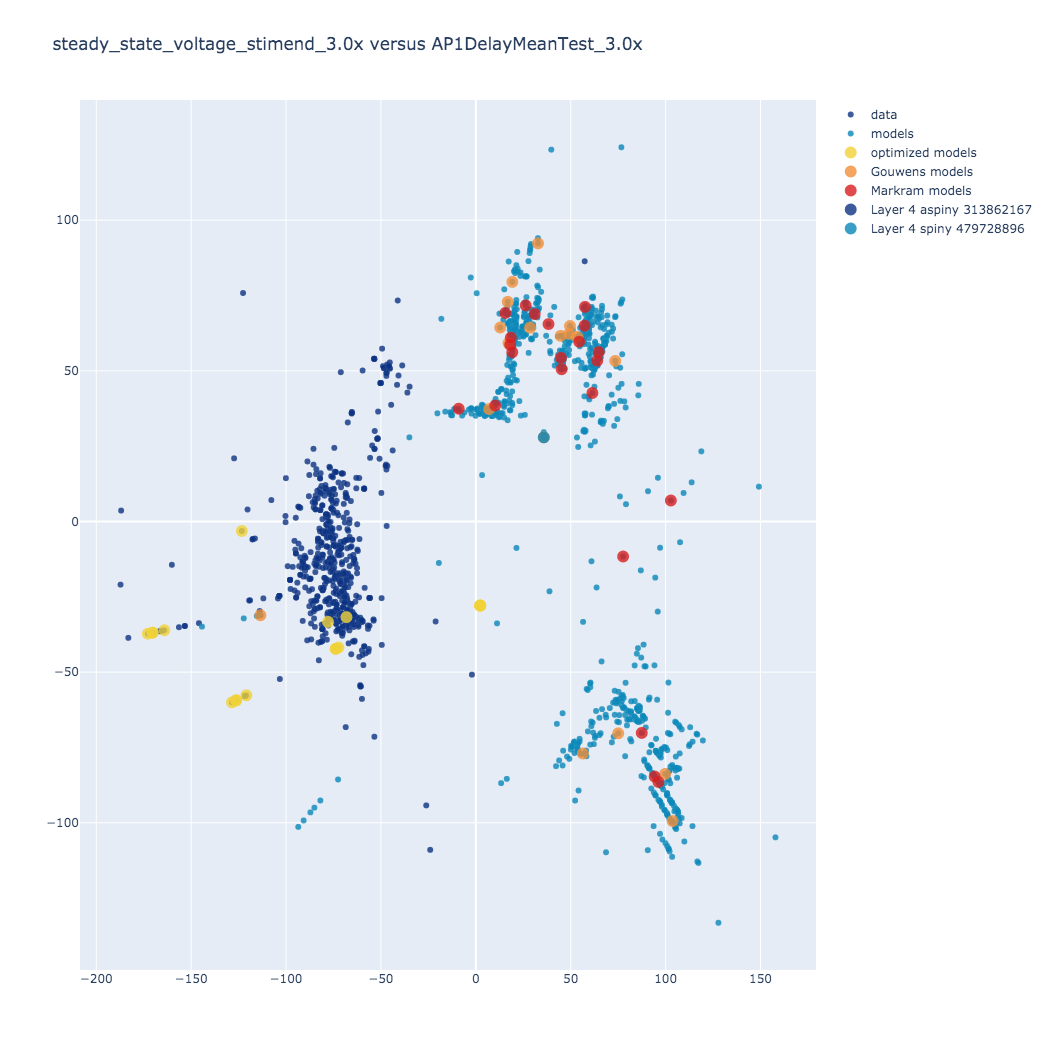
\includegraphics[width=\maxwidth{\textwidth},scale=0.5]{template/PCA.png}
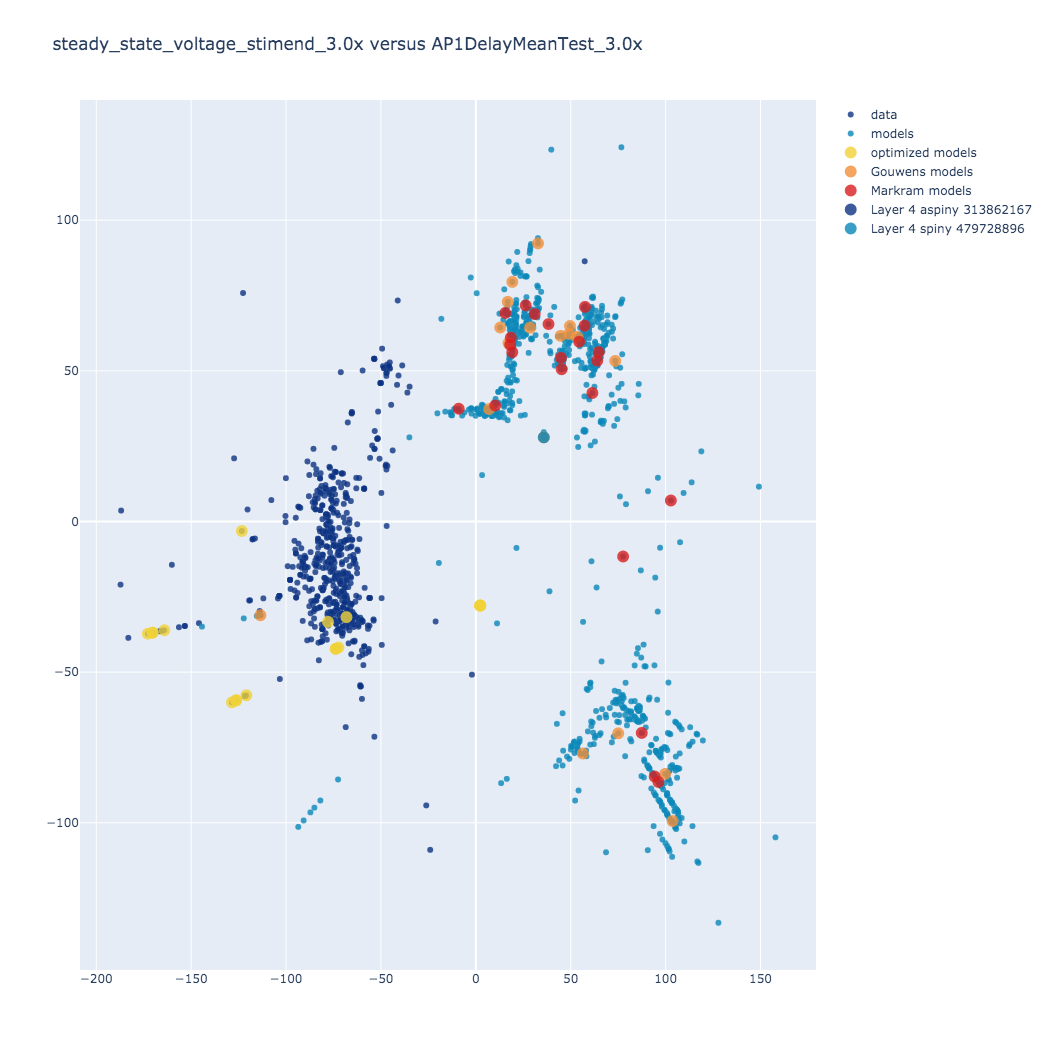
\includegraphics[width=\maxwidth{\textwidth},scale=0.5]{template/PCA.png}
\caption{Principal Component Analysis}
\label{figure\arabic{figurecounter}}
\legend{Feature Variance distributed though-out a plane, the plane was output from applying dimension reduction to a high dimensional (552 dim) feature Space. The plane is related to two projection vectors that were  point in the directions of maximal variance in the data. Data is comprised by a collection of reduced neuronal models, and real recordings of voltage traces from neurons. Data and models are so different in this space that they are easily discriminated, and they fall into several natural clusters. Random Forests variance explained was later used to identify, dimensions that contributed the most variance.
\emph{T-Distributed Stochastic Nearest Neighbour Spatial Embedding} }

\end{figure}




\begin{figure}
\includegraphics[width=\maxwidth{\textwidth}]{figures/TSNE.png}
%\includegraphics[width=\maxwidth{\textwidth}]{template/TSNE.png}
\caption{t distributed stochastic Neigherset Neighbour Spatial Embedding}
\label{figure\arabic{figurecounter}}

\legend{\emph{Source}: \iftoggle{usebiblatex}{\textcite{krishnappa_adult_2012}}{\citet{krishnappa_adult_2012}}}% See:
\legend{\emph{Note}: Here is a note that is especially long to show what happens when it extends to more than one line.}
\end{figure}




\begin{figure}
	\includegraphics[width=\maxwidth{\textwidth}]{figures/TSNE.png}
	\caption{t distributed stochastic Neigherset Neighbour Spatial Embedding}
	\label{figure\arabic{figurecounter}}
\end{figure}

\begin{figure}
	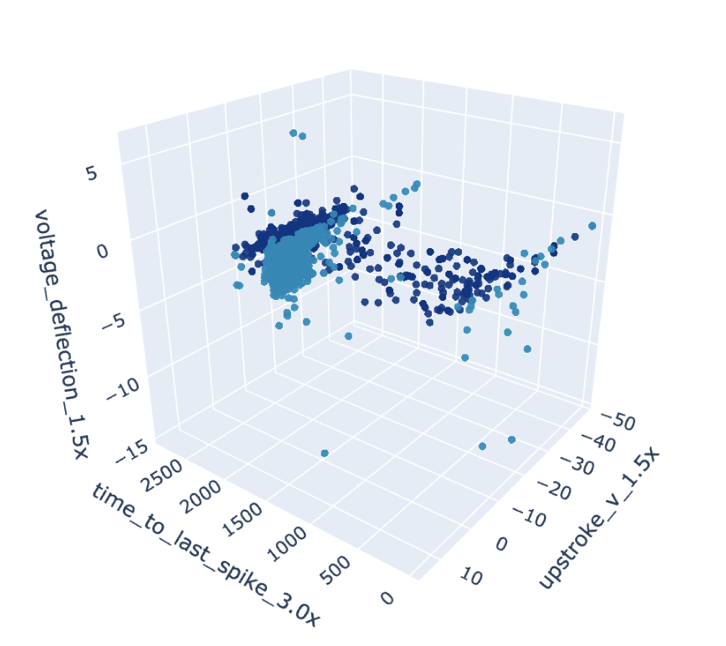
\includegraphics[width=\maxwidth{\textwidth}]{figures/directions_variance.png}
	\caption{t distributed stochastic Neigherset Neighbour Spatial Embedding}
	\label{figure\arabic{figurecounter}}
\end{figure}
\begin{figure}
	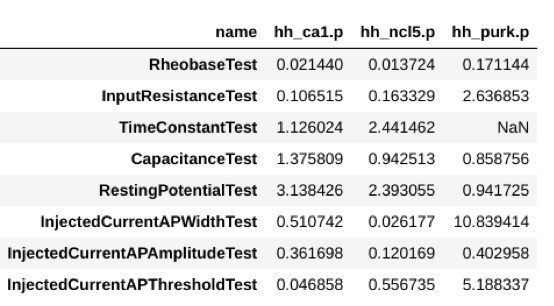
\includegraphics[width=\maxwidth{\textwidth}]{figures/results_conductanc_models.png}
	\caption{t distributed stochastic Neigherset Neighbour Spatial Embedding}
	\label{figure\arabic{figurecounter}}
\end{figure}
\begin{figure}
	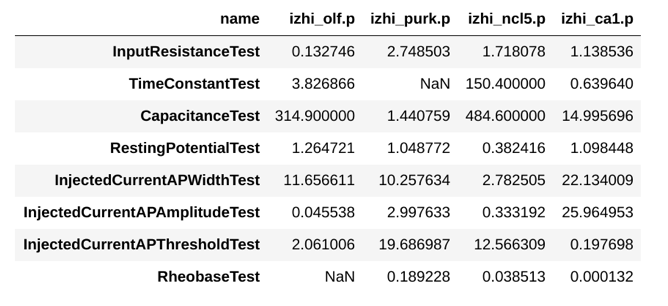
\includegraphics[width=\maxwidth{\textwidth}]{figures/results_izhi_models.png}
	\caption{t distributed stochastic Neigherset Neighbour Spatial Embedding}
	\label{figure\arabic{figurecounter}}
\end{figure}
\begin{figure}
	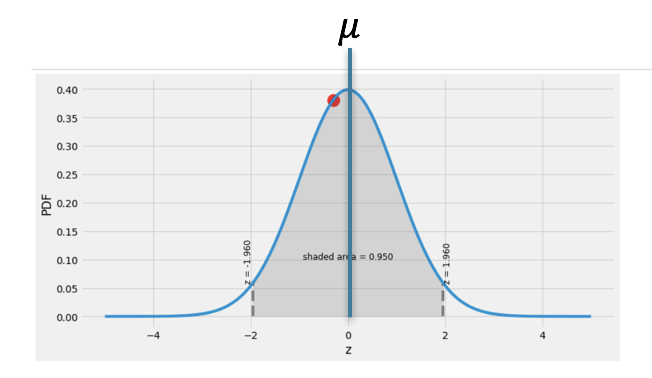
\includegraphics[width=\maxwidth{\textwidth}]{figures/normal_distribution.png}
	\caption{t distributed stochastic Neigherset Neighbour Spatial Embedding}
	\label{figure\arabic{figurecounter}}
\end{figure}
\begin{figure}
	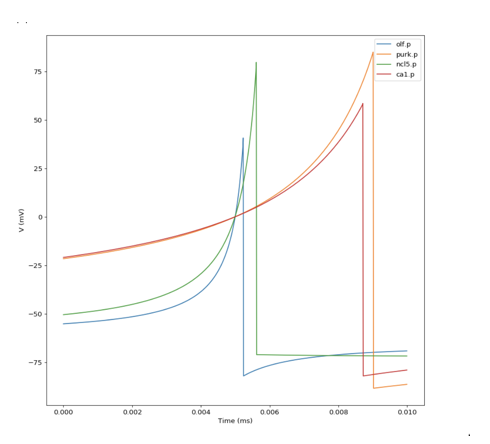
\includegraphics[width=\maxwidth{\textwidth}]{figures/results_izhi_waves.png}
	\caption{t distributed stochastic Neigherset Neighbour Spatial Embedding}
	\label{figure\arabic{figurecounter}}
\end{figure}
\begin{figure}
	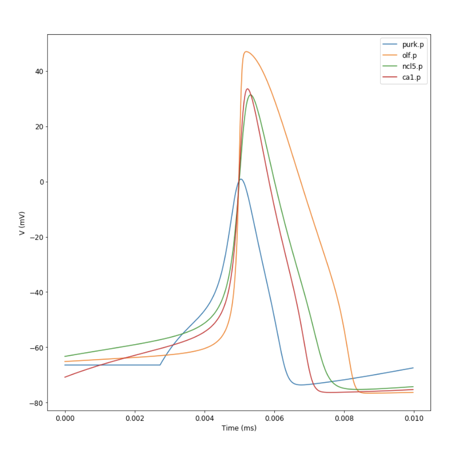
\includegraphics[width=\maxwidth{\textwidth}]{figures/results_conductance_waves.png}
	\caption{t distributed stochastic Neigherset Neighbour Spatial Embedding}
	\label{figure\arabic{figurecounter}}
\end{figure}



\include{template/Optimization_of_existing_models_to_align_them_with_data.tex}
\include{template/Optimization_of_models_to_find_diverse_solutions_for_the_same_behaviors.tex}        
\include{template/Technical_details_of_optimizer.tex}
\include{template/Verification_of_the_optimizer.tex}
%<Insert your chapters here; I recommend to use
%\include{chapter2}                     %   \include rather than \input for chapters
%\include{chapter3}% etc.
                                        % Heading commands (in descending order):
                                        % \chapter
                                        % \section
                                        % \subsection
                                        % \subsubsection
                                        % \paragraph
                                        % \subparagraph
%\iftoggle{sample}{%
%  \chapter{Introduction}

\lipsum[1]

In this research effort, 
\section{Specific Aims}


\subsubsection{1A:} Optimize reduced neuronal models across four different cell types, using two different classes of models:
 
 
 \subsubsection{1B:} By fitting  cellular models to experimental data, using spike waveform shape features,  we can then take optimized models, and characterize and cellular behaviors using Allen SDK and EFEL feature extraction software to evaluate electrical robustness across a large number of features.	

\begin{centre} 
 \begin{tabular}{|c|c|c|c|}
 	\hline 
 	olfactory bulb mitral cell & layer IV pyramidal neuron & cerebellar purkinje cell & ca1 pyramidal cell \\ 
 	\hline 
 	& HH model score &  HH Model score&  HH model score & HH model score\\ 
 	\hline 
 	& Izhikitich model score  & Izhikitich model score & Izhikitich model score& Izhikitich model score \\ 
 	\hline 
 \end{tabular} 
\end{centre} 
 
\citep{searchinger_world_2013}
\refstepcounter{tablecounter}
 


\subsubsection{Aim 2:} Characterize and evaluate region-specific differences of cortical neuron-type data and models.
\subsubsection{2A:} Using large, publicly available datasets for neuron classes, we will characterize region-specific differences and evaluate neuron-type models for agreement with experimental data.
\subsubsection{2B:} Using models of neuron-types from different cortical regions we will identify the features underlying differences among neuron types and across regions, as well as the biophysical mechanisms that underlie those features. 

\subsection{This is the first sub-section-level heading}

\lipsum[1]

\subsubsection{This is the first sub-sub-section-level heading}

\lipsum[1]

\paragraph{This is the first paragraph-level heading}

\lipsum[1]

\subparagraph{This is the first sub-paragraph-level heading}

\lipsum[1]

\section{Citation examples}

The contents of this section differ depending on the bibliography settings, specifically whether the `usebiblatex' toggle is set to `true' or `false'.
\iftoggle{usebiblatex}{%
  This sentence shows citation with biblatex \parencite{searchinger_world_2013}.
  This is another sentence showing citation with biblatex \parencite{pathak_rural_2007}.
}{%
  This sentence shows citation with natbib \citep{pathak_rural_2007}.
  This is another sentence showing citation with natbib \citep{searchinger_world_2013}.
}

\section{Footnote examples}











\refstepcounter{tablecounter}%
%}{}
%%%%%%%%%%%%%%%%%%%%%%%%%%%%%%%%%%%%%%%
% Back matter
%%%%%%%%%%%%%%%%%%%%%%%%%%%%%%%%%%%%%%%
\SingleSpacing                          % Back matter should be single spaced

\edef\defaulttolerance{\the\tolerance}
\tolerance 500                          % Increase tolerance to prevent material extending into margins
\hbadness 500

\iftoggle{useendnotes}{%                % If you're using endnotes, output them here
  \setsecnumdepth{none}                 % No section numbering in end notes
  \printpagenotes
  \setsecnumdepth{all}%                 % Turn section numbering back on after printing
}{}

\chapter*{\bibheading}                  % In the running text, use a chapter-level heading
                                        % for the bibliography section
\phantomsection
\addcontentsline{toc}{chapter}{%        % In the TOC, add a custom chapter-level heading
  \hspace{-\cftchapterindent}%          % that will be flush against the left margin
  \bibheading%
}
%\phantomsection
%\addtocontents{toc}%                    % Add this 'mark' to TOC so subsequent pages use
%  {\protect\markboth{\bibheading}{Page}}%   the bibliography heading (unlikely since
%                                        %   the appendices follow quickly)
\iftoggle{usebiblatex}{%                % Output the bibliography
  \printbibliography[heading=none]      % Using a 'biblatex' package; do not let
                                        %   'biblatex' output a heading
}{%
  \renewcommand\bibsection{}            % Do not let 'natbib' output a heading
  \bibliographystyle{\natbibstyle}      % Using 'natbib' to print bibliography
  \bibliography{\bibfilename}
}

\appendix                               % Indicate start of appendices
                                        % Appendices are considered 'mainmatter' in this
                                        %   documentclass
\tolerance \defaulttolerance            % Set tolerance back to default
\hbadness \defaulttolerance

\addtocontents{toc}{\protect%           % Only include appendix title in table of contents
  \setcounter{tocdepth}{0}}%            %   and omit sub-headings
\renewcommand*{\chapnamefont}%          % Reset font for 'Appendix' in chapter titles
    {\normalfont\MakeTextUppercase}
\makeatletter                           % Clear page after printing appendix title
  \renewcommand{\memendofchapterhook}%
  {%
    \clearpage
    \m@mindentafterchapter
    \@afterheading
  }
\makeatother

\phantomsection                         % Need '\phantomsection' to place hyperref
                                        %   bookmark more accurately
\addcontentsline{toc}{part}{Appendix}   %~Add "Appendix" to TOC here; comment out this
                                        %   line if you're not including appendices

%\phantomsection                        %!This is the one part of the template that I
%\addtocontents{toc}%                   %   could not get to work properly. After you
%  {\protect\markboth{APPENDIX}{Page}}  %   start listing appendices in the TOC,
                                        %   subsequent TOC pages should use "APPENDIX in
                                        %   the header instead of "CHAPTER"; however,
                                        %   this code will make "APPENDIX" appear on the
                                        %   the same page that the *first* appendix
                                        %   appears on. This problem won't affect most
                                        %   people, but if it affects you, uncomment
                                        %   these lines and move them below where
                                        %   the appendices are listed. Keep moving these
                                        %   lines down and checking the output until
                                        %   the TOC headers appear correctly

%\include{appendix1}                     %~Insert your appendices here; I recommend to use
%\include{appendix2}                     %   \include rather than \input for appendices.
%\include{appendix3}% etc.               %   All heading commands are the same as above,
                                         %   e.g., \chapter, \section, etc.
%\iftoggle{sample}{%
%  \chapter{This is a chapter-level heading for an appendix}

\lipsum[1]

\section{This is the first section-level heading in the appendix}

\lipsum[1]

\subsection{This is the first sub-section-level heading in the appendix}

\lipsum[1]

\subsubsection{This is the first sub-sub-section-level heading in the appendix}

\lipsum[1]

\paragraph{This is the first paragraph-level heading in the appendix}

\lipsum[1]

\subparagraph{This is the first sub-paragraph-level heading in the appendix}

\lipsum[1] %
%}{}

\backmatter                             % Start back matter according to documentclass
\makeatletter                           % Do not clear page after printing title for
  \renewcommand{\memendofchapterhook}%  %   biographical sketch
  {%
    \m@mindentafterchapter
    \@afterheading
  }
\makeatother
%\chapter{Biographical Sketch}           %~Biographical Sketch is optional
%\input{biography}                       %<Enter the name of the .tex file containing your
                                        %   biography or omit this line and type in
                                        %   your biography here (1 paragraph)
                                        
                                        


\end{document}
